\section{Ratatouille, a tool for understanding RemyCCs}

In our experience, high-performing computer-generated
congestion-control algorithms present a different kind of complexity
than existing mechanisms. Traditional TCP congestion control schemes
specify relatively simple rules for each endpoint, but the resulting
emergent behavior of a multiuser network is not easily specified and
can be suboptimal and unstable. By contrast, Remy's algorithms specify
hundreds of rules at the endpoints, but produce more consistent
overall behavior.

We think this tradeoff is ultimately worth taking: today's endpoints
can execute complex algorithms almost as easily as simple ones, and
the \textit{computational} complexity of a RemyCC is low in any
event. But when endpoint algorithms become so complex, it is
challenging to explain why a particular RemyCC works without
considerable effort spent reverse-engineering it. To help with this
task, I built a visualization and debugging tool for RemyCCs, called
Ratatouille.

Ratatouille displays real-time output from the Remy network simulator,
and plots the current number of packets-in-flight for each concurrent
flow as it evolves over time. The user adjusts a physical USB control
surface (a software mixing board) to vary network parameters,
including the number of flows with offered load and the link rate,
propagation delay, and buffer size at the bottleneck queue. The user
can then observe how the flows respond to the changing
conditions. Ratatouille can also run conventional AIMD TCP-like flows
for comparison.

By exploring the evolving values of the congestion signals, we have
gained some intuition into how a RemyCC can achieve good
performance. When the network is in steady state, the congestion
signals of a RemyCC sender tend to fall into an orbit, or limit cycle,
in which the average number of packets-in-flight over the cycle is
close to the ``ideal'' number: the bandwidth-delay product of the
bottleneck link divided by the degree of multiplexing.

The period of the limit cycle is generally a small number of RTTs. By
contrast, TCP's congestion window generally oscillates on a much
longer timescale that depends on the buffer size, because the
``multiplicative decrease'' feature of TCP's control rules is only
triggered when packet loss is detected, typically only after buffer
overflow occurs in the bottleneck queue.

Our observations suggest that a RemyCC's ability to achieve better
throughput than TCP on finite-length flows is mostly due to its
quicker response to changes in conditions---a RemyCC will generally
``ramp up'' to the ideal number of packets-in-flight more quickly than
the TCP slow-start algorithm (Figure~\ref{fig:ratscreen}).

Although Ratatouille has allowed us to make observations that suggest
``why'' RemyCCs achieve their good performance compared with
human-designed mechanisms, much more work will be necessary before we
can reason about the performance and robustness of RemyCCs in a
rigorous way.

\begin{figure}
\caption{Ratatouille allows a user to vary network conditions on a
  physical control service, then observe the resulting behavior of a
  RemyCC in real-time. Below, the initial startup and steady-state
  behavior of the RemyCC-100x algorithm of Section~\ref{s:oprangeperftradeoff}.}
\label{fig:ratscreen}

\begin{center}

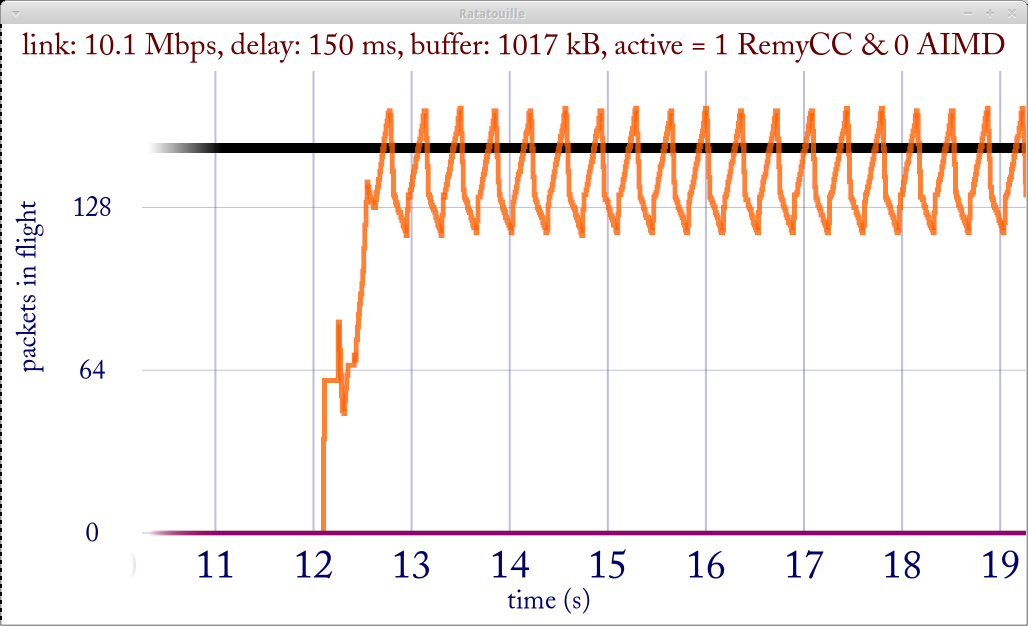
\includegraphics[width=0.85 \textwidth]{ratatouille.png}

\end{center}
\end{figure}
